\chapter{Assoziationsdatenbank und Website}
Der Hauptteil von TIMA ist die Datenbank in denen die Assoziation gespeichert werden. Diese ist direkt verknüpft mir dem Webfrontend, dass sowohl der Hauptanlaufpunkt für die Benutzer ist als auch für die Apps durch die Bereitstellung einer umfassenden API.

Im nächsten Abschnitt wird das Backend und die Datenbank genauer beschrieben. Dabei wird genauer auf den Aufbau der einzelnen Tabellen eingegangen, sowie die verschiedenen Designentscheidungen.

Anschließend wird die API und die dahinter stehenden Designentscheidung genauer erläutert.

\section{Backend und Datenbank}
Für das Backend der Website haben für Django als grundlegende Technologie entschieden. Bei Django handelt es sich um ein in Python geschriebenes Webframework, das dem Model-View-Controller-Schema folgt. Django bietet unter anderem einen sehr komplexen objektrelationalen Mapper, der es ermöglicht auch komplexe Objektstrukturen abzubilden ohne die verwendete Datenbank explizit zu kennen.

\subsection{Datenmodell}
In \hyperref[fig:uml]{Abbildung \ref*{fig:uml}} ist das komplette Datenmodell von TIMA dargestellt. Dabei bildet das Modul \texttt{associations.models} den Kern.

\begin{figure}
	\centering
	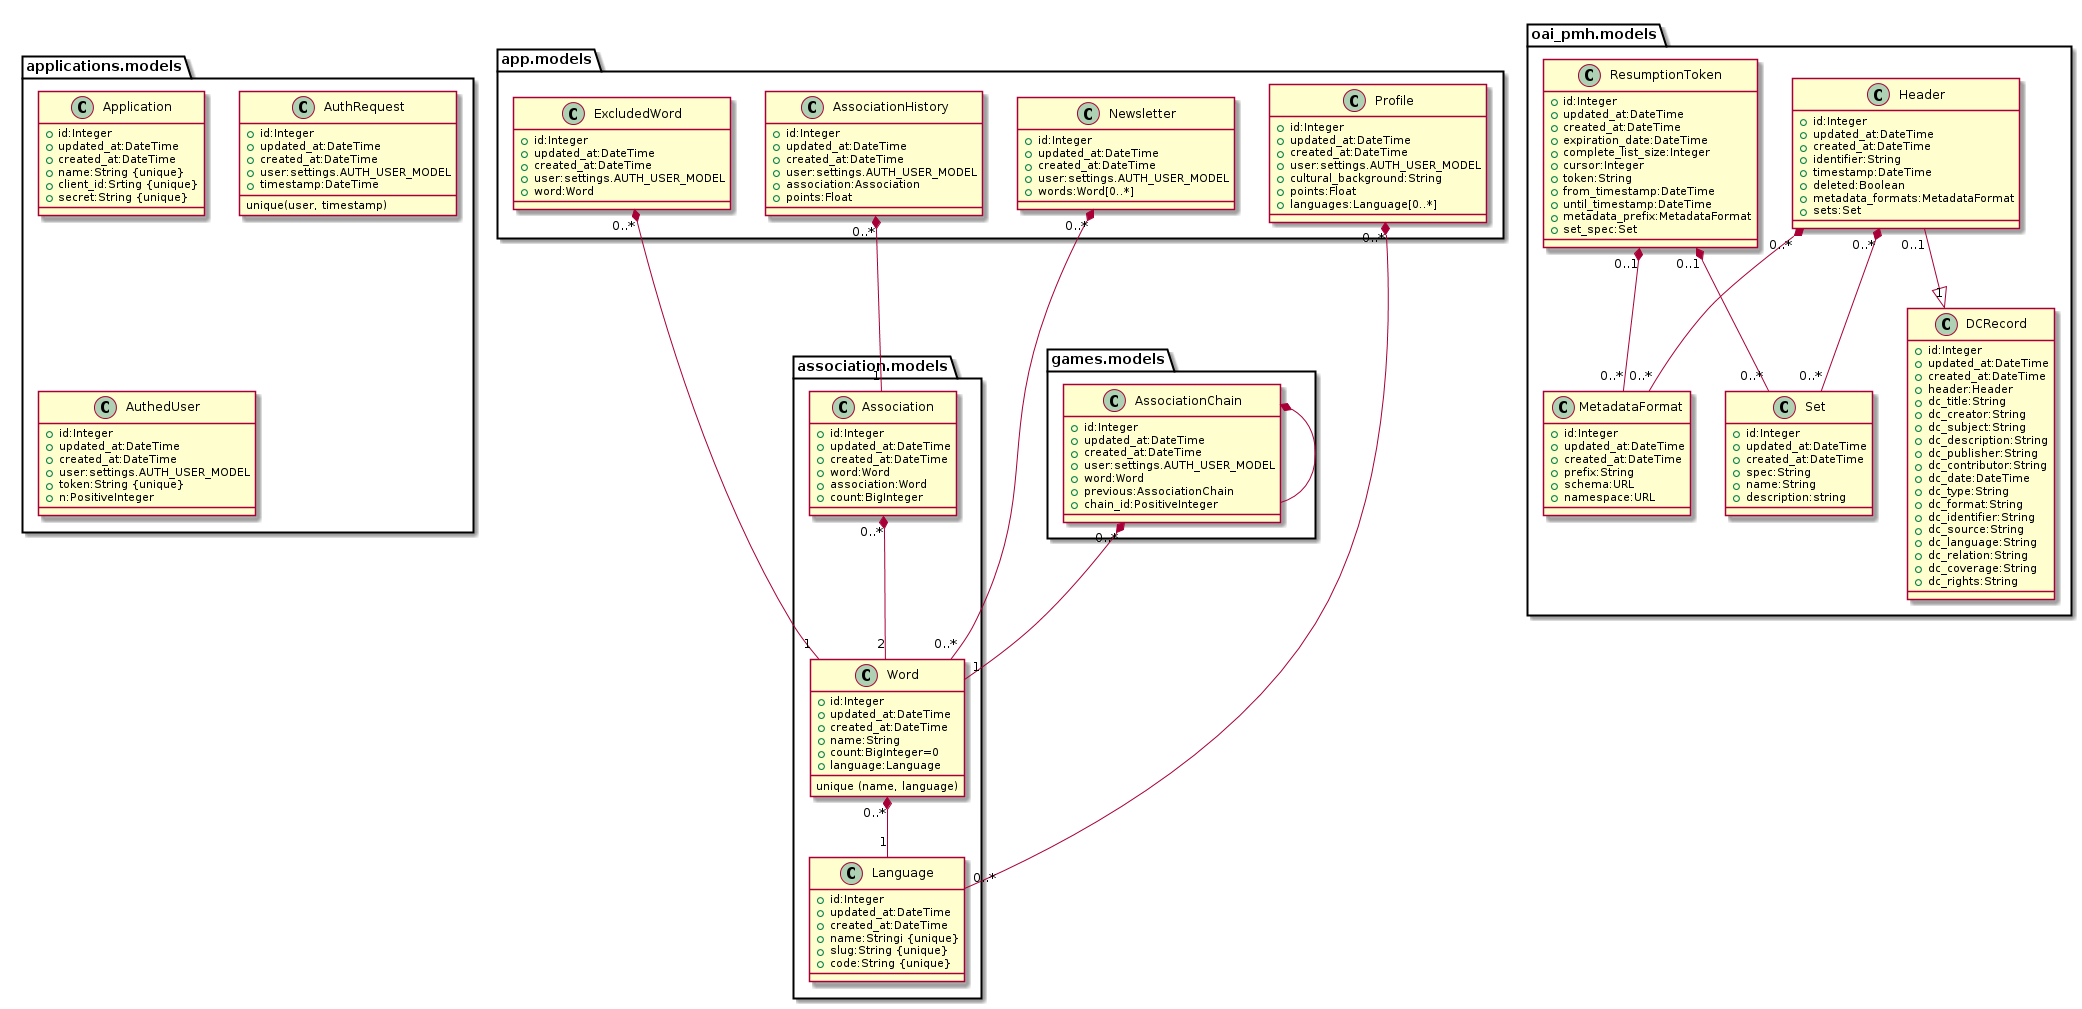
\includegraphics[width=\textwidth]{images/uml.png}
	\caption{UML des TIMA Datenmodells}
	\label{fig:uml}
\end{figure}

Das Modell \texttt{Language} repräsentiert die verfügbaren Sprachen der Wörter, das Modell \texttt{Word} die einzelnen Wörter, wobei ein Wort, wenn es in mehreren Sprachen existiert, für jede Sprache einen eigenen Eintrag hat und das Modell \texttt{Association} die Assoziation zwischen zwei Wörtern. Zusätzlich wird bei einem Wort gespeichert, wie oft dieses gefragt wurde und bei der Assoziation wir häufig diese gegeben wurde.

Die Modelle des Moduls \texttt{app.models} behandeln grundlegende Funktionen des Benutzermanagements. So zum Beispiel das Modell \texttt{Profile}, dass den Kulturellen Hintergrund, die Punktzahl und die Sprachen für die ein Benutzer assoziiert hat, speichert. In dem Modell \texttt{AssociationHistory} wird die gesamte Assoziationsgeschichte eines Benutzers gespeichert, mit den jeweils für eine Assoziation erhaltenen Punkte. Das Modell \texttt{ExcludeWord} enthält für jeden Benutzer die Wörter, die er übersprungen hat (siehe TODO ref), diese werden automatisch nach sieben Tagen gelöscht. Das letzte Modell in diesem Modul speichert für jeden Benutzer welche Worte er in seinem Newsletter empfangen möchte.

Das Modul \texttt{games.models} enthält Modelle die für verschiedenen Spiele wichtig sind. Dies ist im Moment nur AssoziationsKette (vgl. TODO ref), hierfür werden in dem Modul \texttt{AssociationChain} die letzte/aktuelle Assoziationskette eines Benutzer gespeichert. Diese wird bei jedem Start eines Spieles gelöscht.

Für die Kommunikation zwischen App und Backend, insbesondere die schreib Zugriffe (vgl. TODO ref), zu autorisieren und dem speichert der nötigen Informationen dient das Modul \texttt{applications.models}. Das Modell \texttt{Applicaion} speichert die Apps, die Autorisiert sind, mit den nötigen Daten für die Autorisierung (vgl TODO ref). Die beiden anderen Modell in diesem Modul \texttt{AuthRequest} und \texttt{AuthedUser} speichern die nötigen Information für einen Benutzer der sich authentifizieren möchte und hat.

Das letzte Modul und die beinhalteten Modell sind für das OAI-PMH erforderlich siehe dafür (TODO ref).

\section{Webfrontend}
Das Webfrontend ist die Hauptanlaufstelle für Benutzer. Hierüber kann sowohl anonym als auch angemeldet Assoziationen eingegeben, Wörter und deren Assoziationen angesehen und weitere Funktionen (Rangliste, Statistik) aufgerufen werden.

Das Webfrontend basiert auf Django, wurde zusätzlich zu HTML mit Bootstrap und JQuery erstellt, sowie zur Visualisierung D3.

\section{API}
Damit die verschiedenen Apps mit der TIMA Datenbank kommunizieren können, haben wir uns entschieden eine umfangreiche API zu implementieren. Diese lässt sich grob in drei Teile. Zum einen gibt es die Anfragen, die keiner Autorisierung bedürfen, zweitens jeden die einer Autorisierung erfordern und drittens eine OAI-PMH Schnittstelle.

Eine komplette Dokumentation der API ist in der Datei API.md\footnote{\url{https://github.com/Tima-Is-My-Association/TIMA/blob/master/API.md}} im git zu finden.

Im folgenden Abschnitt werden die einzelnen API Anfragen die keiner Autorisierung bedürfen näher erläutern, im darauffolgenden Abschnitt die, die eine Autorisierung benötigen, dort wird ebenfalls der Autorisationsprozess näher erläutert. Zum Schluss wird dann noch ein Abschnitt zu OAI-PMH folgen.

\subsection{Nicht autorisierte Anfragen}
\subsection{Autorisierte Anfragen}
Zum einem soll man sich über die Apps auf die Anmelden können, zum anderen soll nicht jede beliebige App schreib zugriff auf die TIMA Datenbank haben. Aus diesem war er erforderlich, dass einige API Anfragen einer Autorisation bedürfen.

Um dies zu realisieren haben wir uns zunächst bestehende Frameworks wie zum Beispiel OAuth2 angeschaut und getestet in wie weit diese unseren Anforderungen genügen. Dies hat allerdings zu keinen zufriedenstellendem Ergebnis geführt, weswegen wir entschieden haben dies selbstständig zu implementieren.

Die grundlegenden Anforderungen die wir dabei hatten sind wie folgt:
\begin{enumerate}
	\item sichere Authentisierung einer App
	\item sichere Authentisierung eines Benutzers
	\item sicherstellen das spätere Anfragen von einem Authentisierten Benutzer kommen
\end{enumerate}

\begin{figure}
	\centering
	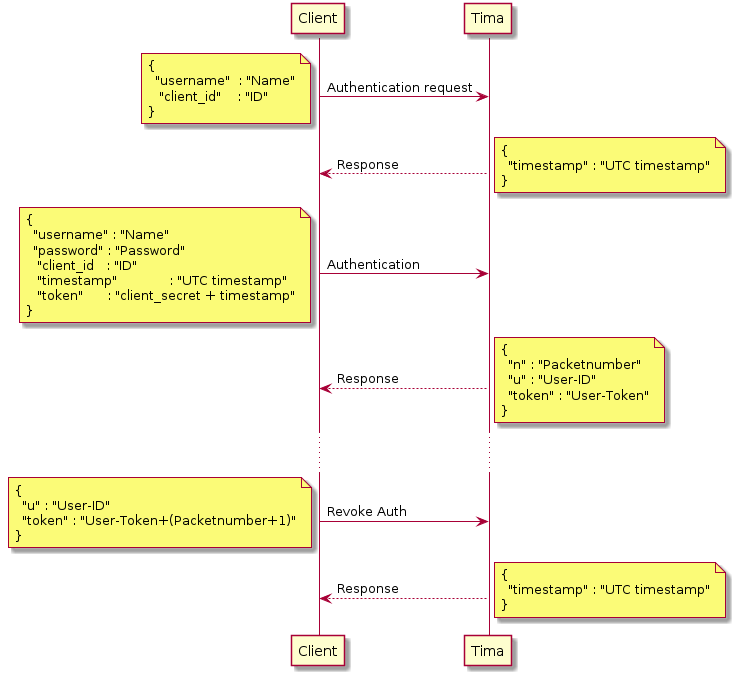
\includegraphics[width=\textwidth]{images/auth.png}
	\caption{Authentisierungsprozess}
	\label{fig:auth}
\end{figure}

In \hyperref[fig:auth]{Abbildung \ref*{fig:auth}} ist der Authentisierungsprozess schematisch Dargestellt. Der Client ist dabei eine App, ber die sich ein Nutzer authentisieren möchte. Die App verfügt zum einen über eine \texttt{client\_id} und über ein \texttt{secret}, beides von TIMA vergebene eindeutige zufällige Strings. Der Authentisierungsprozess läuft wie folgt ab.
\begin{enumerate}
	\item Eine App sendet eine Anfrage an TIMA mit dem \texttt{username} des Benutzers und der \texttt{client\_id}. TIMA prüft diese beiden Werte auf Existenz und antwortet entweder mit \textbf{200} (HTTP Response Code) und dem aktuellen Zeitstempel oder mit \textbf{404}.
	\item Als nächstes sendet die App die eigentliche Authentisierungsanfrage. Mit \texttt{username} und \texttt{password} des Benutzers, \texttt{client\_id} der App, dem Zeitstempel der Antwort der letzten Anfrage und einem \texttt{token} das aus dem \texttt{secret} der App und dem Zeitstempel geniert wird (SHA512).
	\item TIMA antwortet wenn die Authentisierung erfolgreich war mit \textbf{200} und den folgenden drei Werte:
	\begin{itemize}
		\item[n] Paketnummer jeden Anfrage einer App muss diese um eins nach oben zählen. Als Wertebereich ist uint32 zubenutzen.
		\item[u] eine eindeutige Benutzer-ID, die bei jeder Anfrage mit zusenden ist
		\item[token] einem zufälligen String der bei jeder Anfrage zusammen mit \texttt{n}, der Paketnummer, in einem SHA512 Hash zu senden ist
	\end{itemize}
\end{enumerate}

\subsection{OAI-PMH}
bisschen OAI-PMH
